\section{Background and Motivation}

\begin{figure}[t]
    \centering
    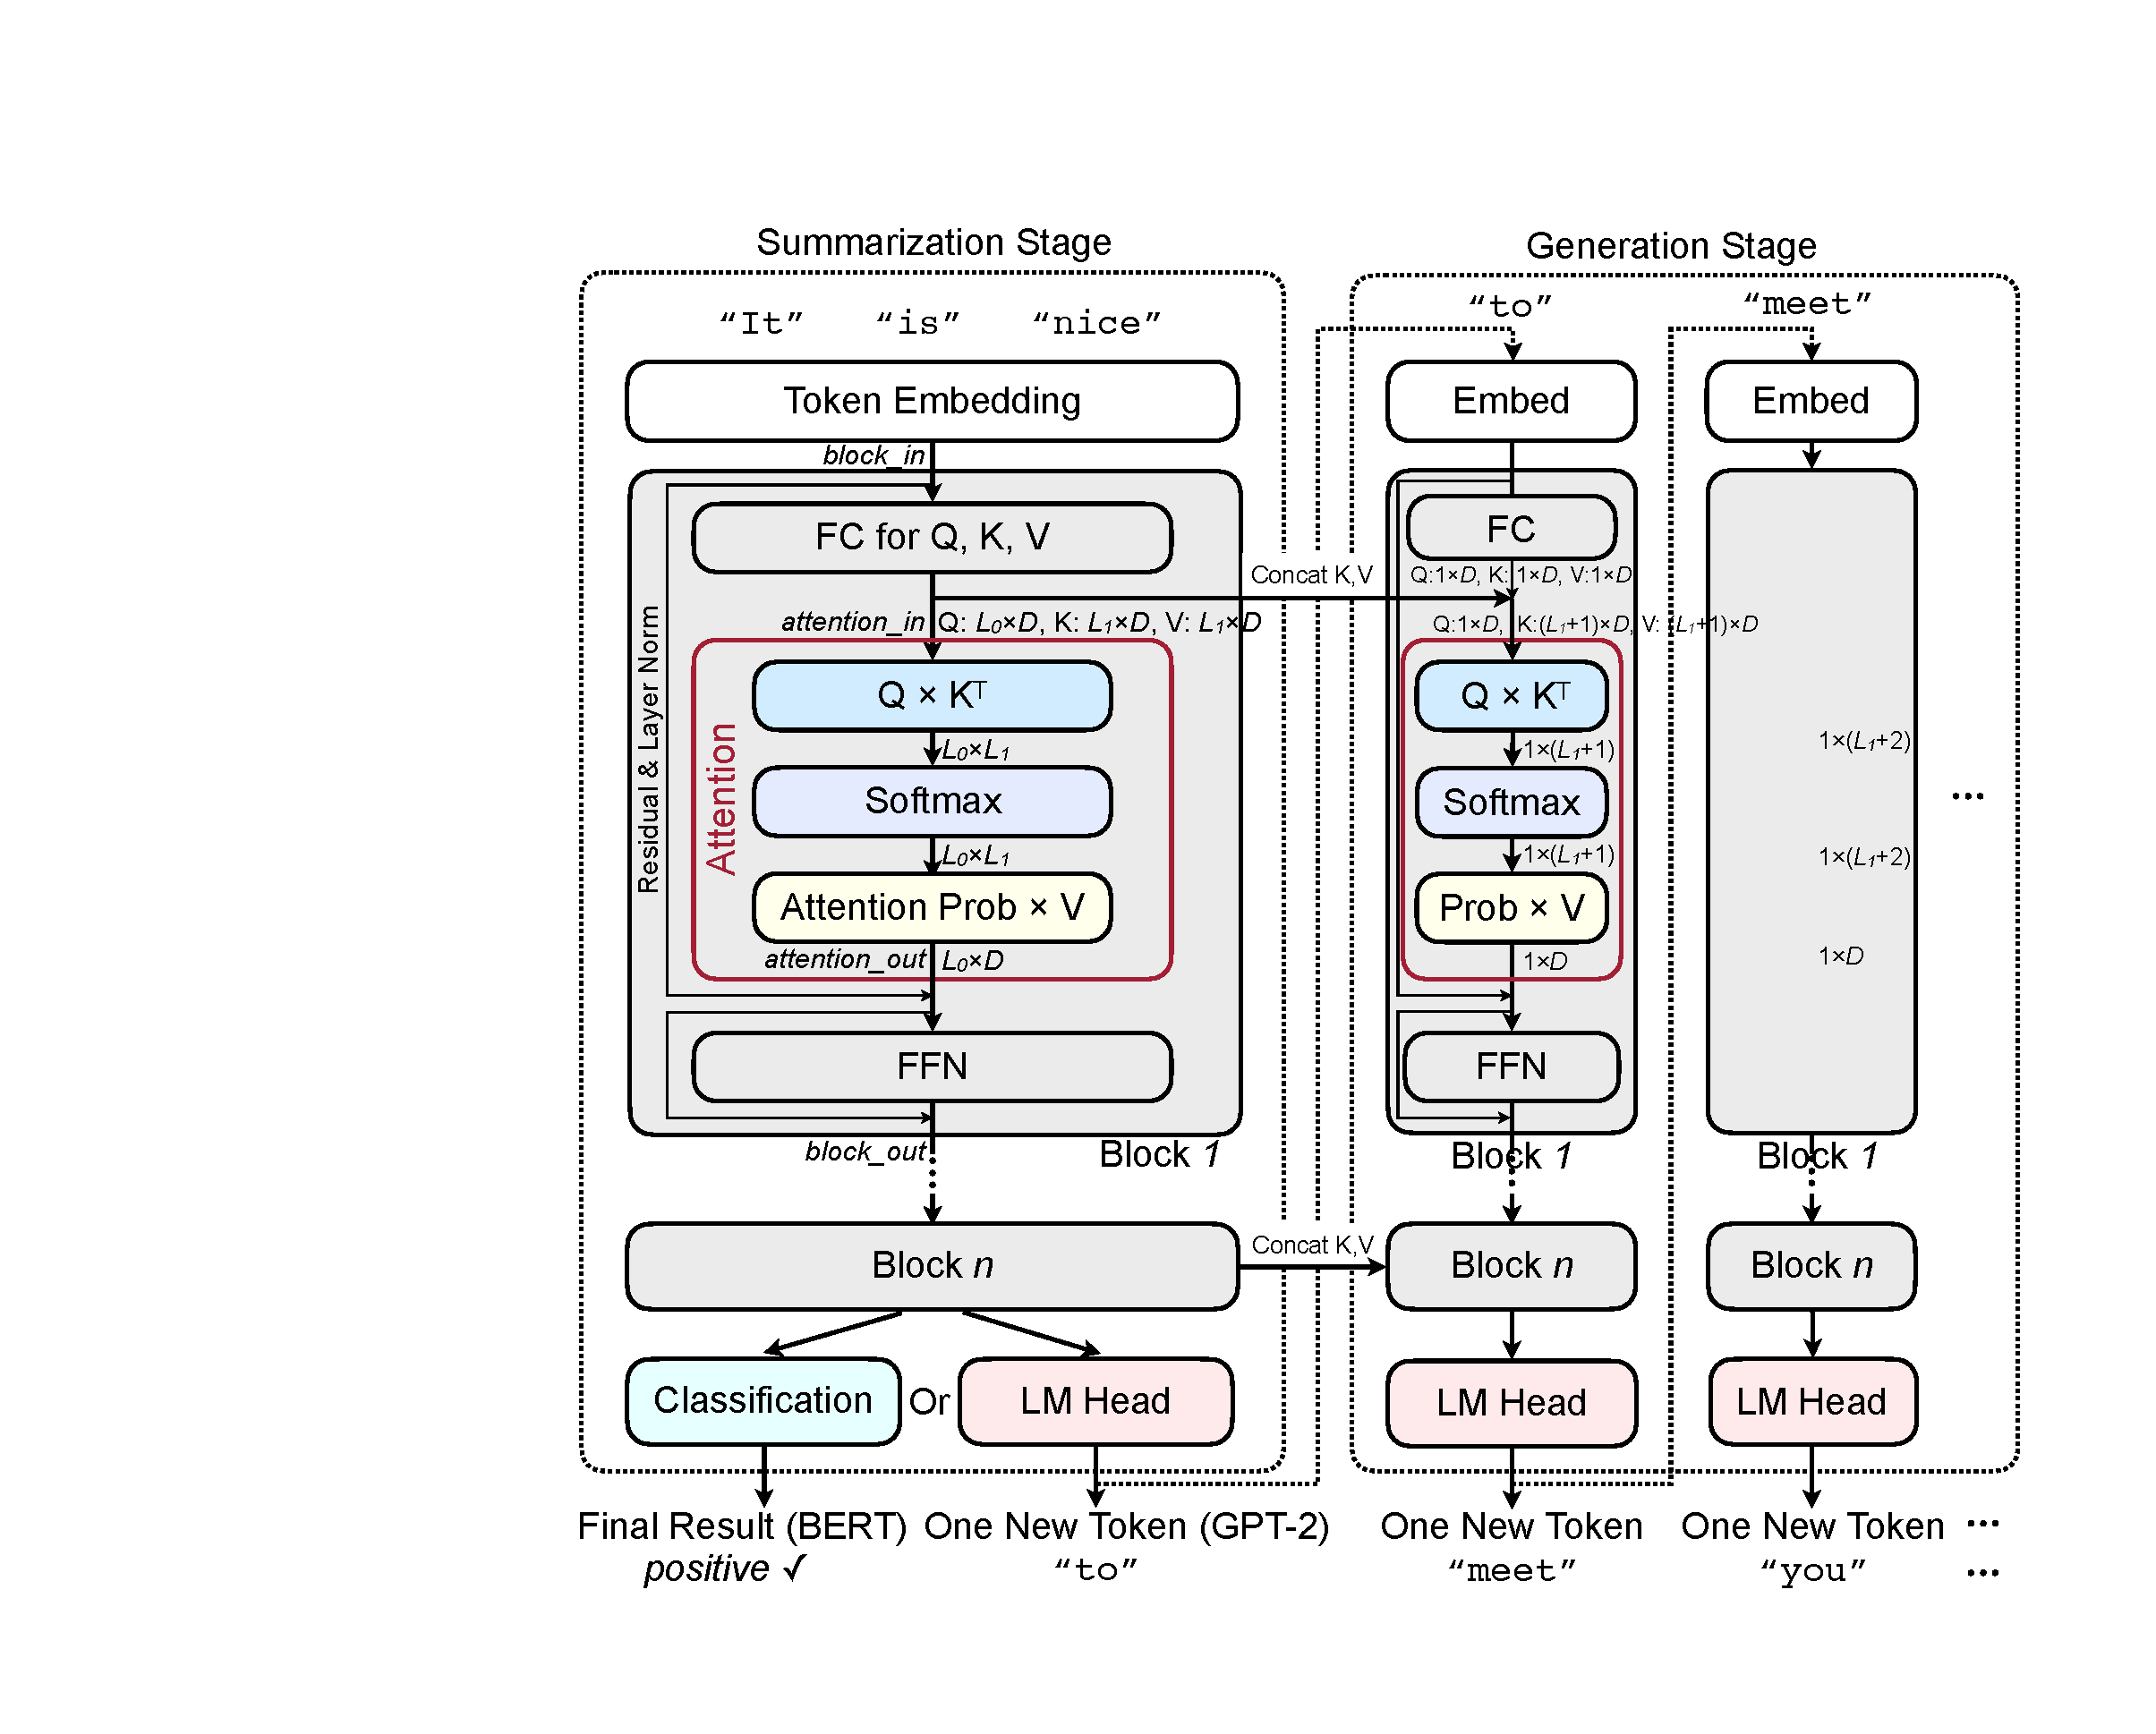
\includegraphics[width=\columnwidth]{figures/background.pdf}
    \vspace{-15pt}
    \caption{NLP model architecture with attention. \bert only contains the summarization stage. \gpttwo contains summarization and generation stages.
}
    
    \label{fig:background}
\end{figure}

\newlength{\oldtextfloatsep}\setlength{\oldtextfloatsep}{\textfloatsep}

\setlength{\textfloatsep}{0pt}
\begin{algorithm}[!t]
\SetKwInOut{Input}{Input}
\footnotesize{
    \SetAlgoLined
    \textbf{Input:} 
    $Q_{in} \in \mathbb{R}^{L_0 \times D_{in}}$,
    $K_{in} \in \mathbb{R}^{L_1 \times D_{in}}$, 
    $V_{in} \in \mathbb{R}^{L_1 \times D_{in}}$; \\ 
    Number of Heads: $h$ ; \\
    Split $Q_{in}, K_{in}, V_{in}$ to $h$ chunks:  \\
    $
    Q \in \mathbb{R}^{ h \times L_0 \times D}, K \in \mathbb{R}^{ h \times L_1 \times D},  V \in \mathbb{R}^{ h \times L_1 \times D}, D = \frac{D_{in}}{h} $; \\
    \For{$head_{id} = 0 \mathbf{ \ to \ } h$}{
    
    \colorbox{qxkcolor}{\vbox{ 
    $attention\_score \in \mathbb{R}^{  L_0 \times L_1}$ ;\\ 
    $attention\_score = Q[head_{id}] \cdot K[head_{id}]^T $ ;\\
    $attention\_score = attention\_score /$sqrt($D$) ; \\
    }}
    
    \colorbox{softmaxcolor}{\vbox{ 
    $attention\_prob \in \mathbb{R}^{  L_0 \times L_1}$ ;\\
    \For{$row_{id} = 0 \mathbf{ \ to \ } L_0$}{
    $attention\_prob[row_{id}] = $ Softmax($attention\_score[row_{id}]$)
    }
    }}
    
    \colorbox{probxvcolor}{\vbox{ 
    $E[head_{id}] = attention\_prob \cdot V[head_{id}]$ ;\\
    }}
    
    }
    
    Concatenate heads of $E \in \mathbb{R}^{ h \times L_0 \times D}$ as output; \\
    \textbf{Output:} $attention\_out \in \mathbb{R}^{L_0 \times D_{in}}$;\\
    
    \caption{Attention}
    }
    \label{algo:attention}



\afterpage{\global\setlength{\textfloatsep}{\oldtextfloatsep}}

\end{algorithm}

\subsection{Background}
\textbf{Attention-Based NLP Models.}
NLP tasks can be categorized into two types: discriminative and generative. For discriminative ones, the models need to summarize the input information and make predictions. Discriminative tasks include token-level classification\cite{tjong-kim-sang-de-meulder-2003-introduction}, sentence-level classification and regression~\cite{socher-etal-2013-recursive} \etc 
Meanwhile, models for generative tasks need first to summarize the input information and then generate new tokens. Exemplary generation tasks include Language Modeling (LM)~\cite{radford2019language} and machine translation~\cite{46201}.

\bert for discriminative and \gpttwo for generative tasks are the most widely-used models as illustrated in  Figure~\ref{fig:background}. \bert only contains the summarization stage, while \gpttwo contains summarization and generation stages. In summarization (Figure~\ref{fig:background} left), the input tokens are first embedded into vectors and processed by blocks. Inside each block, $block\_in$ are first multiplied with three matrices to get Query (Q), Key (K) and, Value (V). Then QKV are processed by attention to get the intermediate features $attention\_out$. A residual layer adds the $attention\_out$ with $block\_in$ and conducts layer normalization. There will be an additional FC on $attention\_out$ if there is more than one head. Furthermore, a Feed-Forward Network (FFN) layer containing two Fully-Connected (FC) layers is applied. Finally, another residual operation is conducted and outputs $block\_out$.
The same block is repeated multiple times such as 12 times for \bert-Base. The last block is followed by one classification layer in \bert to get the \emph{final result}. In contrast, \gpttwo applies an LM head to generate one new token and enters the generation stage.

Generation stage (Figure~\ref{fig:background} right) has two main differences from summarization: 1) Each iteration only processes \emph {one single token} instead of the whole sentence. 2) Ks and Vs from the summarization stage are concatenated with current K and V, and sent to attention \emph{in batch}, while the query is still \emph{one single vector}. After the last block, another new token will be generated. Generation stage ends when \texttt{end\_of\_sentence} token is generated, or the sentence length reaches a pre-defined limit. One generation iteration's runtime is similar to the whole summarization stage on GPU, because the summarization is processed in batch.

\begin{figure*}[t]
    \centering
    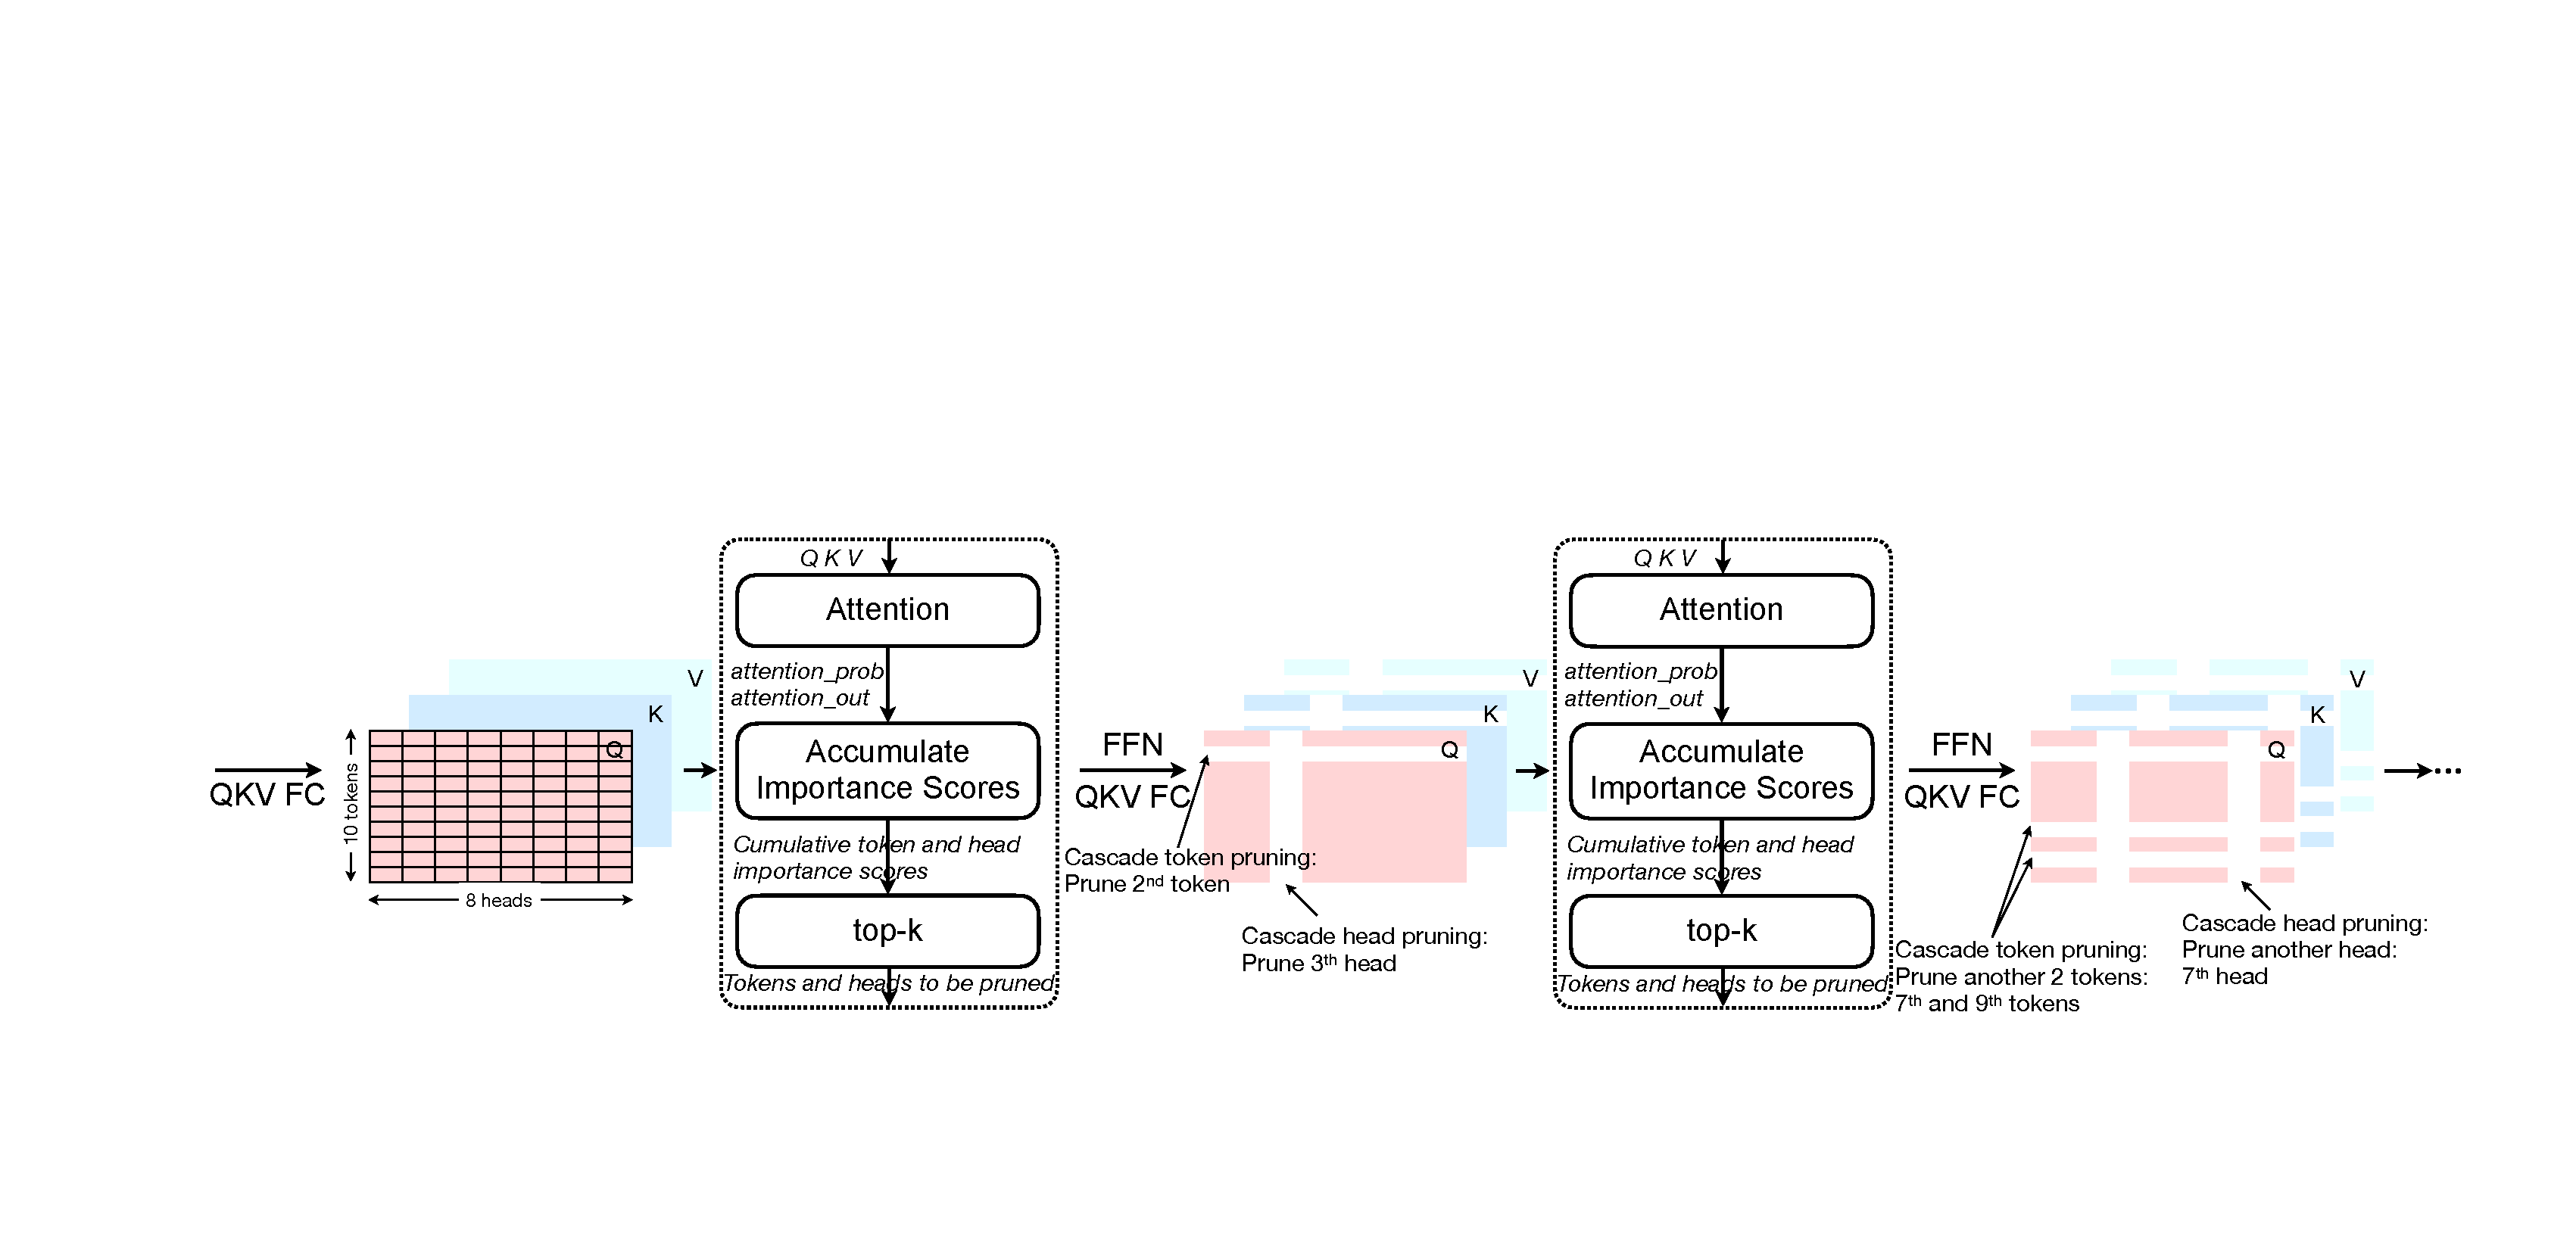
\includegraphics[width=1\textwidth]{figures/methodology.pdf}
    \vspace{-15pt}
    \caption{Cascade token pruning removes redundant tokens and corresponding entire Q K V vectors according to the cumulative token importance scores computed from $attention\_prob$. Cascade head pruning removes unimportant heads and corresponding chunks in all Q K V vectors according to the cumulative head important scores computed from $attention\_out$. Once a token/head is pruned, it will never appear in any following layers, thus named cascade pruning. More tokens and heads are pruned away as the layer goes deeper.}
    \vspace{-15pt}
    \label{fig:methodology}
\end{figure*}

\setlength{\textfloatsep}{0pt}

\begin{algorithm}[!t]
\footnotesize{
\SetKwInOut{Input}{Input}
    \SetAlgoLined
    \textbf{Input:} 
    Number of heads: $h$;\\
    Token pruning ratio: $p_{t}$; Head pruning ratio: $p_{h}$;\\
    $attention\_prob \in \mathbb{R}^{ h \times L_0 \times L_1}$, 
    $attention\_out \in \mathbb{R}^{L_0 \times D_{in}}$; \\
    Previous cumulative token importance score: $s_{t} \in L_1;$ \\
    Previous cumulative head importance score: $s_{h} \in h;$
    
    Reshape $attention\_out$ by head, get $E \in \mathbb{R}^{ h \times L_0 \times D}$;
    \tcc{accumulate the token importance}
    \For{$token_{id} = 0 \mathbf{ \ to \ } L_1$}{
        \For{$l_{0} = 0 \mathbf{ \ to \ } L_0$}{
            \For{$head_{id} = 0 \mathbf{ \ to \ } h$}{
                $s_{t}[token_{id}] \mathrel{{+}{=}} attention\_prob[head_{id}][l_0][token_{id}]$
            }
        }
    }
    \tcc{accumulate the head importance}
    \For{$head_{id} = 0 \mathbf{ \ to \ } h$}{
        \For{$l_{0} = 0 \mathbf{ \ to \ } L_0$}{
            \For{$d = 0 \mathbf{ \ to \ } D$}{
                $s_{h}[head_{id}] \mathrel{{+}{=}} abs(E[head_{id}][l_0][d] )$
            }
        }
    }
    
    $remained\_token\_id = $ top-k($s_t, L_1 \times (1-p_t)$) \\
    $remained\_head\_id = $ top-k($s_h, h \times (1-p_h)$) \\
    
    \textbf{Output:} $remained\_token\_id, remained\_head\_id, s_t, s_h$
    
    \caption{Token and Head Pruning (one layer)}
}
    \label{algo:cascade}
\afterpage{\global\setlength{\textfloatsep}{\oldtextfloatsep}}
\end{algorithm}






\textbf{Attention Mechanism.} The attention mechanism~\cite{46201} is shown in Algorithm~\ref{algo:attention}. In the summarization stage, Q, K, and V are matrices with the same dimension, while in the generation stage, Q is one single vector, and K, V are matrices. 

Attention has multiple \textit{heads}, each processing a chunk of Q, K, and V. Different heads capture various dependencies between tokens, some for long-term, some for short-term. Inside each head, $\mathrm{Q} \times \mathrm{K}^{T} / \mathrm{sqrt}(D)$ gives attention scores, which indicate whether two tokens are related. For instance in Figure~\ref{fig:heatmap_bert}, the score for `more' attending to `than' is large. After that, a row-wise softmax computes the attention probabilities. The exponential of softmax further enlarges the score for highly-related token pairs. The head's feature is then computed with $attention\_prob \times$V. This step lets each token fetch information from their cared tokens. Finally, multiple heads are concatenated together as the attention output. In \bert-Base and \gpttwo-Small, there are 12 blocks, and each attention layer has 12 heads. There are 24 blocks and 16 heads for each attention layer in \bert-Large and \gpttwo-Medium.



\subsection{Motivation}
\label{sec:motivation}
We profile the end-to-end latency of a \gpttwo model on multiple hardware platforms in Figure~\ref{fig:latency_breakdown}. Attention typically accounts for over 50\% latency, even though it only has around 10\% of overall \flops. In Figure~\ref{fig:latency_breakdown} right, around 73\% of the time is spent on data movements such as splitting heads, K and V concatenations, reshape, and transpose. 
GPUs and CPUs are well-optimized for matrix multiplications but are poor on the complex memory operations, thus slowing down attention. Therefore, it is necessary to build an accelerator to solve the attention bottleneck as a co-processor. The FC layers of NLP models are processed by GPUs, CPUs, or tensor algebra accelerators as they are highly-optimized for FC, and our \name co-processor handles all attention layers.

\begin{figure}[t]
    \centering
    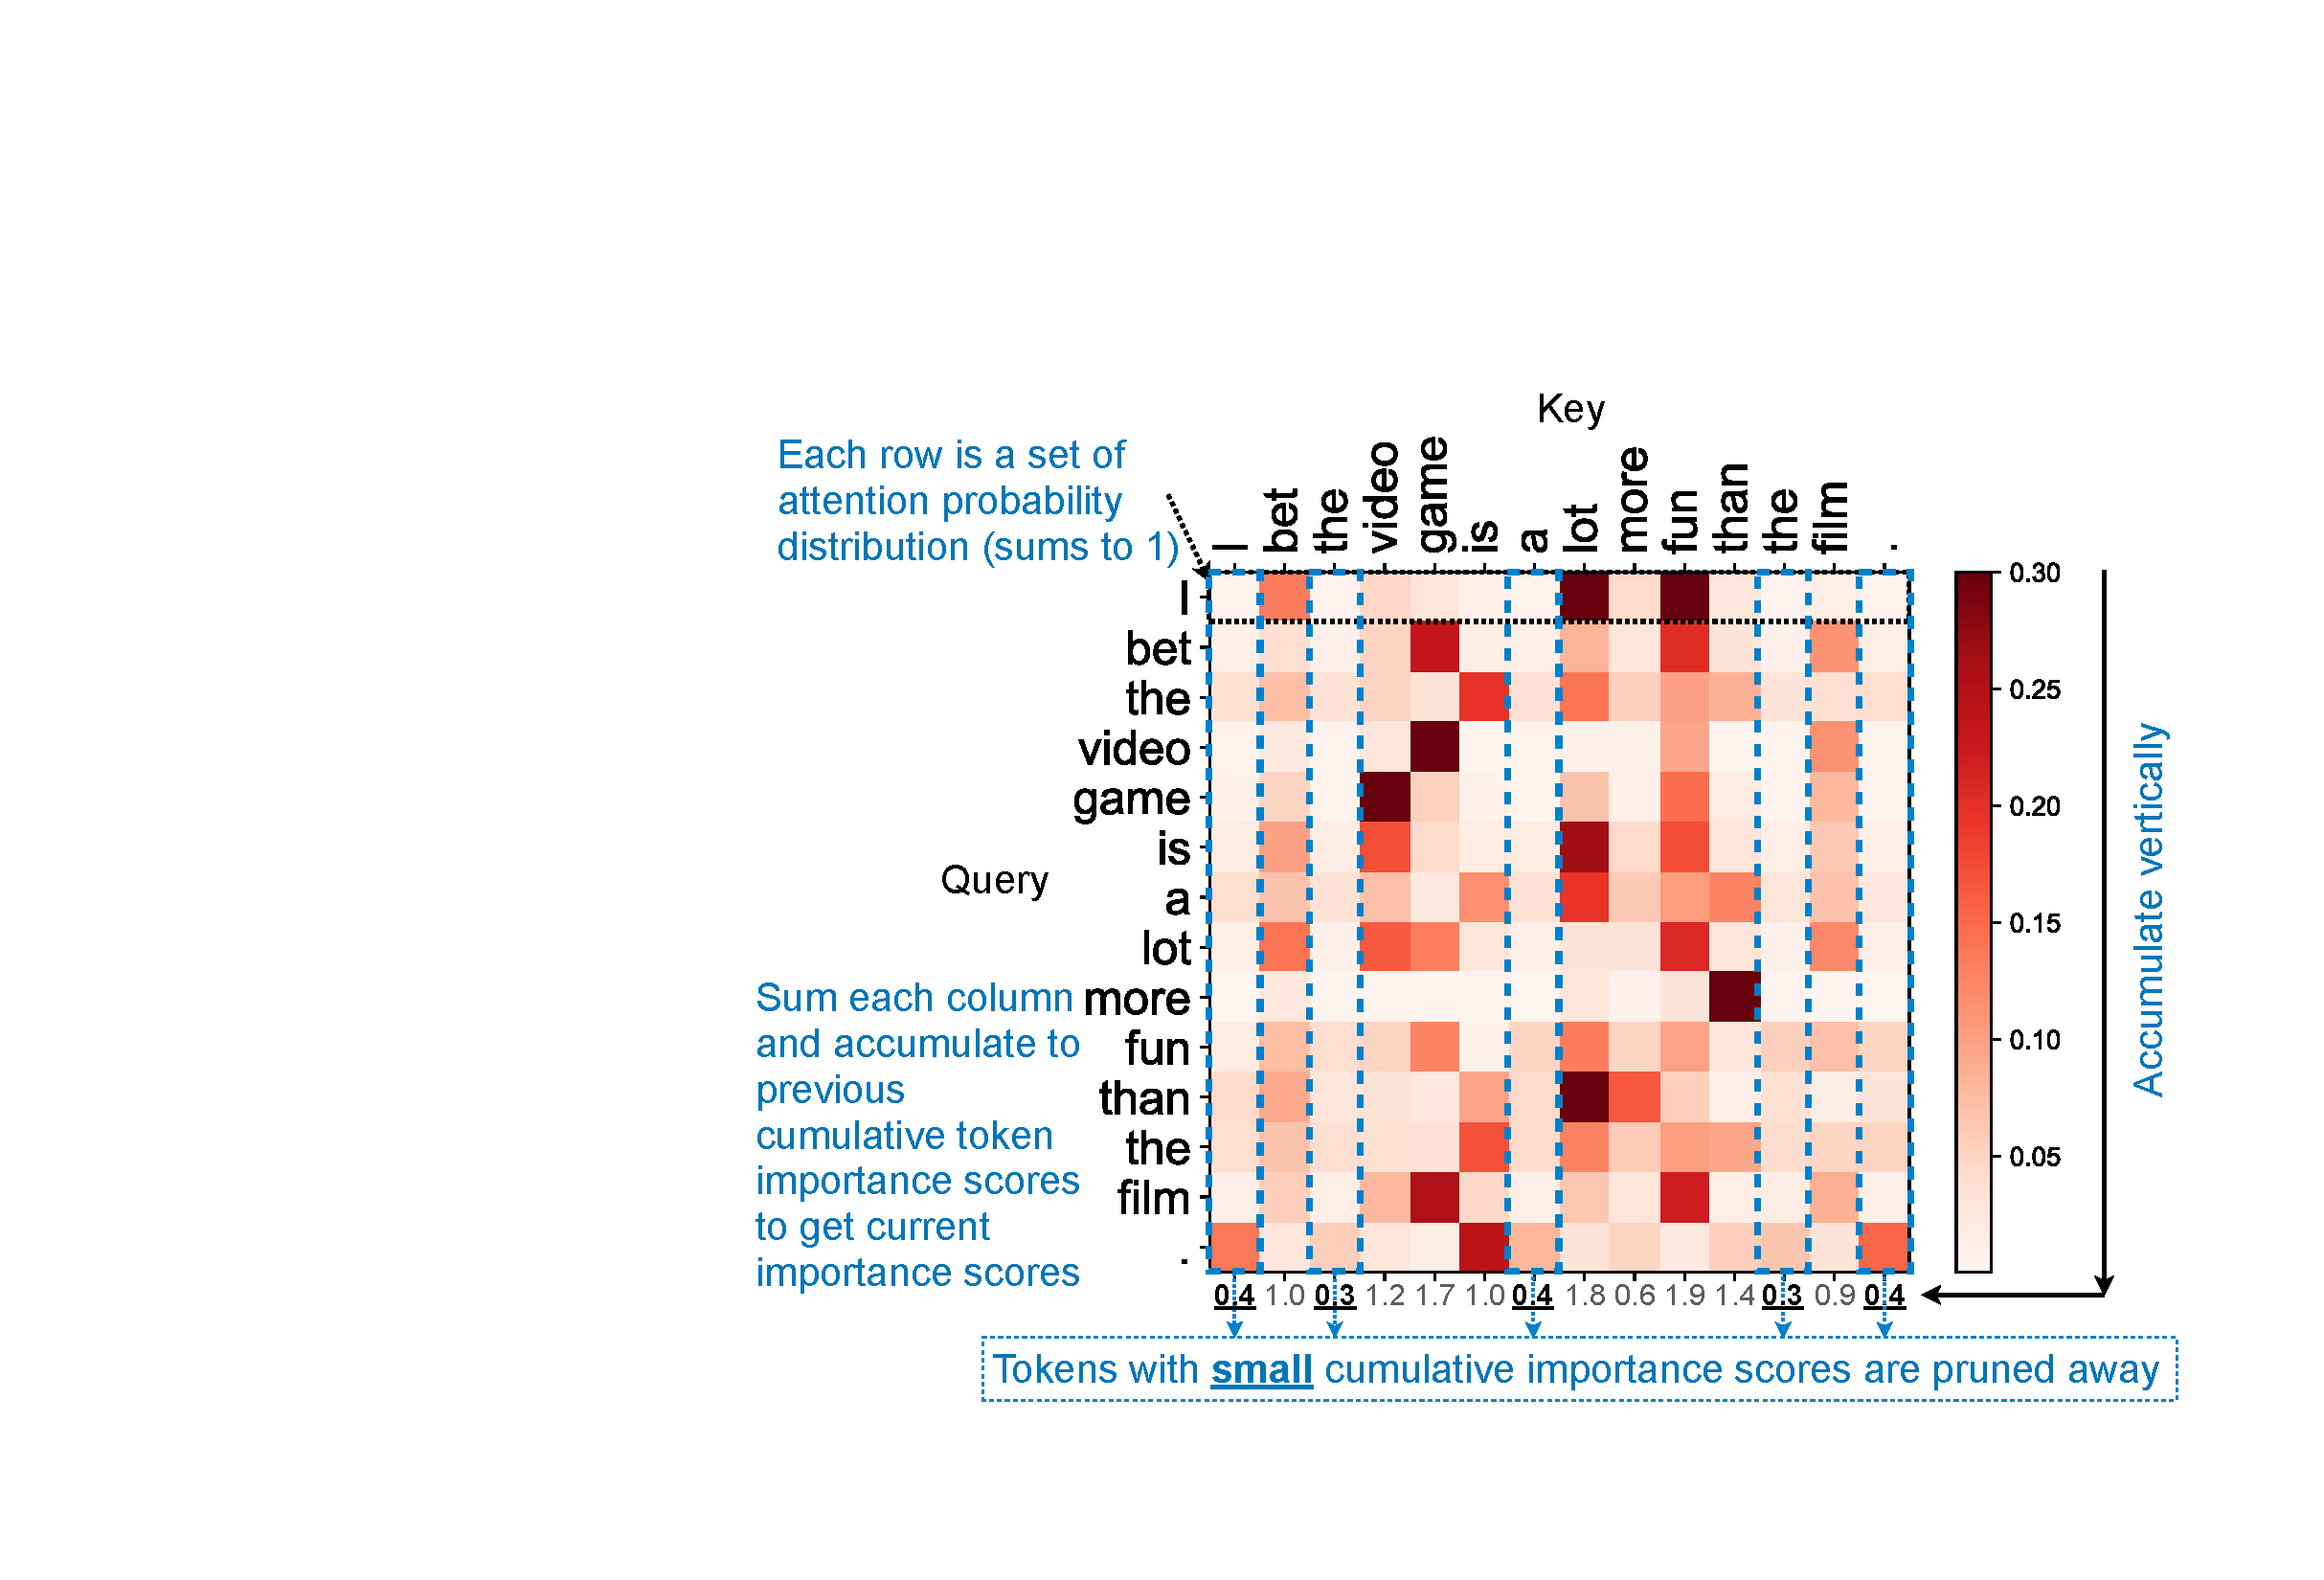
\includegraphics[width=\columnwidth]{figures/heatmap_bert.pdf}
    \vspace{-10pt}
    \caption{Attention probabilities for \bert are summed over each column to get importance scores. Tokens with small importance scores are pruned.}
    \vspace{-10pt}
    \label{fig:heatmap_bert}
\end{figure}


